\subsection{Audio Tone Start Detection}
\subsubsection{Background Research}
Detection of when a tone starts is a very important feature when trying to accurately measure distance. If the start of the tone is not accurately measured, the measured travel time of the tone will not be accurate, resulting in an inaccurate distance measurement.\\

There are many different solution within the music industry in detecting when a audio tone begins. Often these solution fall into one of two categories, a very simple solution errors greater than $1ms$, or requires a significant amount of processing time to successfully detect the tone if done on a Limpet.\\

A more appropriate solution for achieving distance measurements was found. This solution is often used in tasks of distance measurement, for example Sonar and Ultrasonic Sensors \cite{toa_akeem_2020}. The solution is to use convolution to find the a specific "chirp" within an audio recording, this "chirp being a linear FM sweep.

\subsubsection{Convolution Implementation}
The linear FM sweep "chirp" hs the form shown in Figure \ref{fig:linear_fm_sweep}, this specific example is not scale. A "chirp" is a sweep from one frequency to another frequency over a period. The specific configuration often used during testing while implementing the method is a linear FM sweep from 1kHz to 2kHz over 1 second.

\begin{figure}[H]
	\centering
	\noindent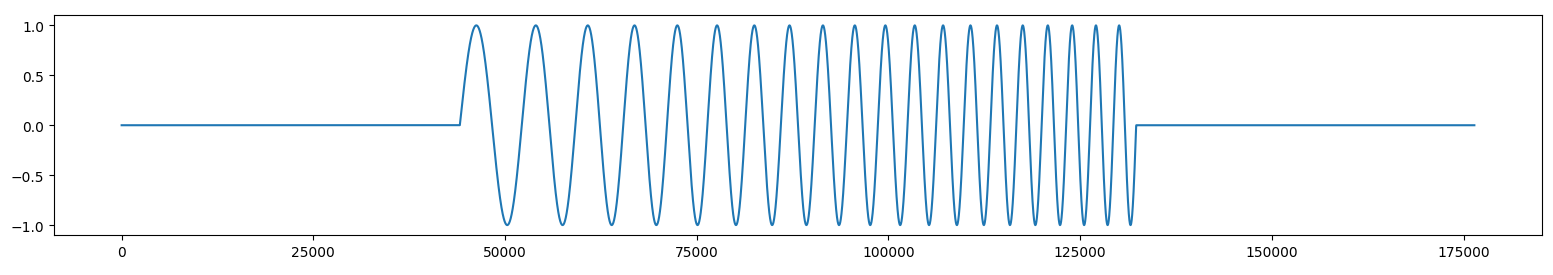
\includegraphics[width=0.95\textwidth]{images/linear_fm_sweep.png}
	\caption{An example of what a linear FM sweep looks like}
	\label{fig:linear_fm_sweep}
\end{figure}

The actual implementation of the linear FM sweep with using convolution is shown in Figure \ref{fig:matched_filter}. The top graph is the output signal to the speakers, the middle graph is the audio recording, and the bottom graph is the output of the convolution. The vertical orange line is the guessed start location in the received audio recording. During testing there was a variation of $\pm 30mm$ in distance measurements at a constant 240mm distance. This variation can be converted into a variation in time, being $\pm 0.1ms$. Further testing will be required to correctly profile this method of distance measurement, as the platform used for testing didn't guarantee accurate time measurements.

\begin{figure}[H]
	\centering
	\noindent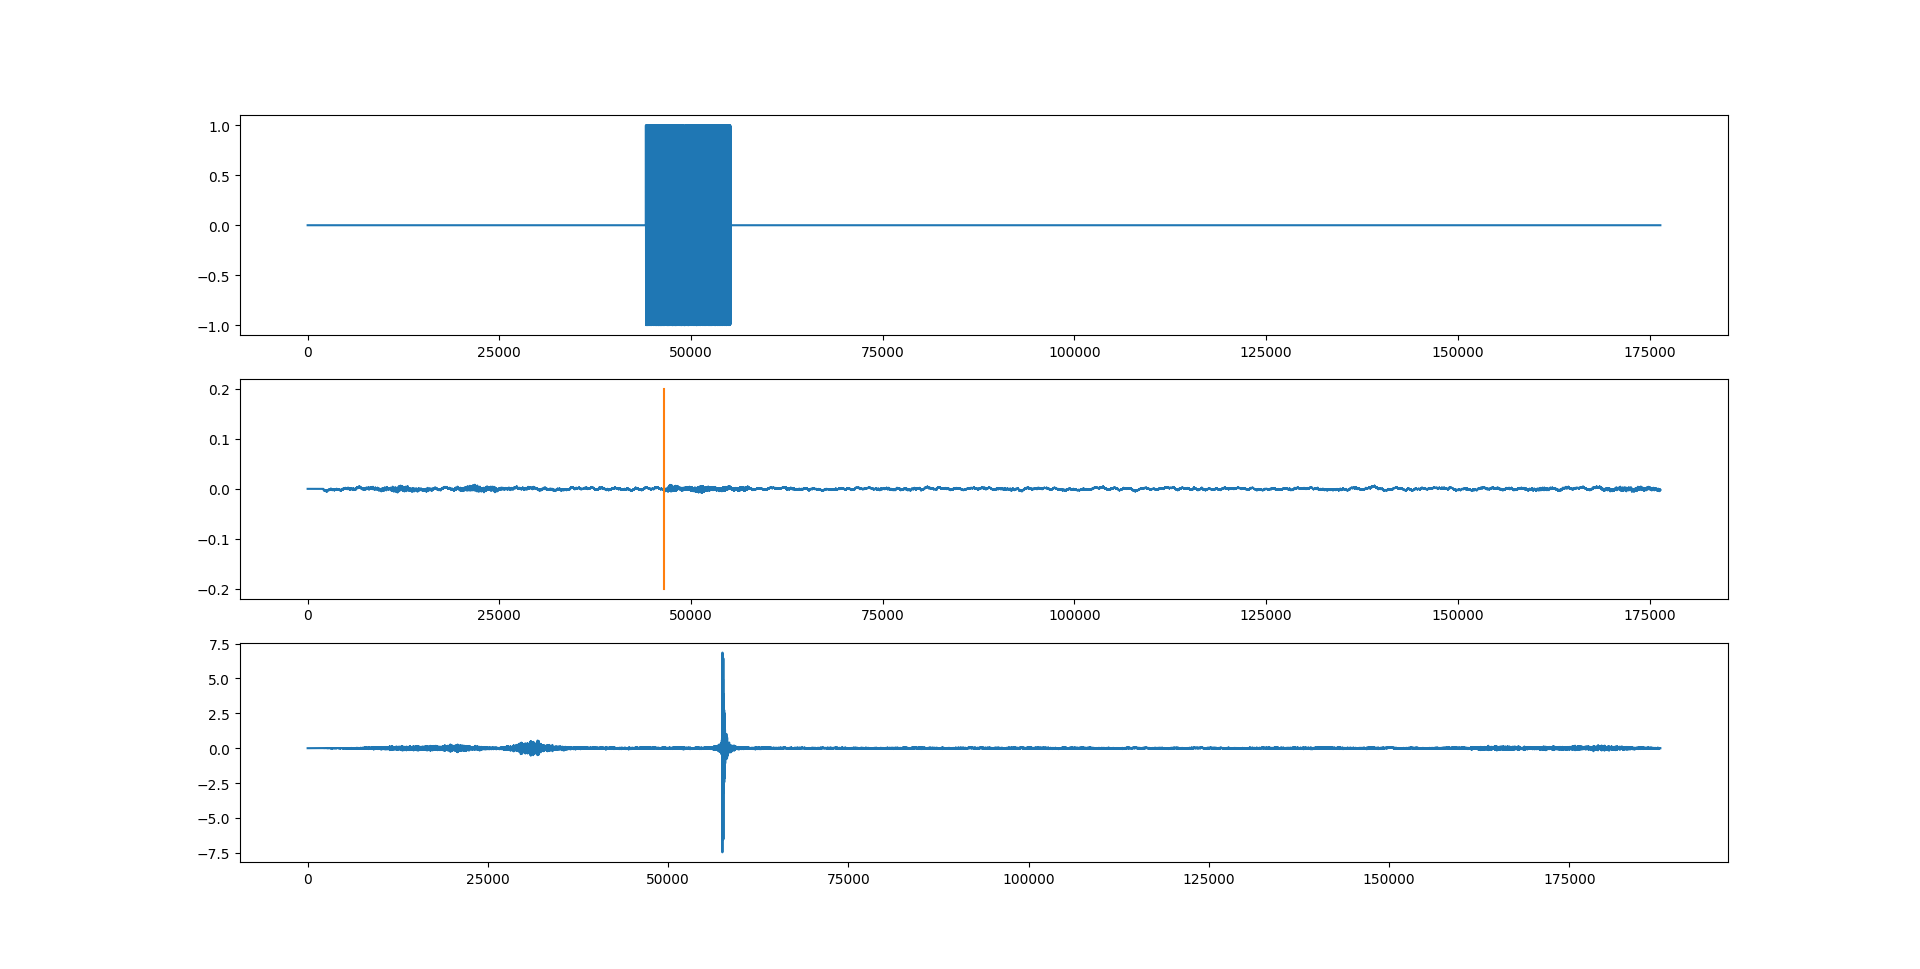
\includegraphics[width=0.95\textwidth]{images/matched_filtering.png}
	\caption{An example of what a linear FM sweep looks like}
	\label{fig:matched_filter}
\end{figure}



\subsection{Distance Measurement}
Measuring distance between two points using sound requires recording how long a sound takes to travel between the points. Ultrasonic distance sensors do this by sending out a tone that bounces back off an object and records how long it took the sound to travel the round trip, this time is halved to get a one-way trip period. The one-way trip period is then used to calculate the distance based off the speed of sound.\\

The limpet's cannot physically bounce a sound off of another limpet as the limpets cannot control the direction of emitted sound. This limitation means that the limpets cannot individually measure the distance between themselves and other limpets.\\

The first approach to measuring distance is to use the inbuilt Real Time Clock (RTC) of the controller within the limpet. In a system of two limpets, one limpet would be programmed to emit a sound at a specific time and the other limpet would start recording how long it has been since a sound was emitted. Figure \ref{fig:limpetOneway} is a visualisation of how the one way communication works.\\

\begin{figure}[H]
	\centering
	\noindent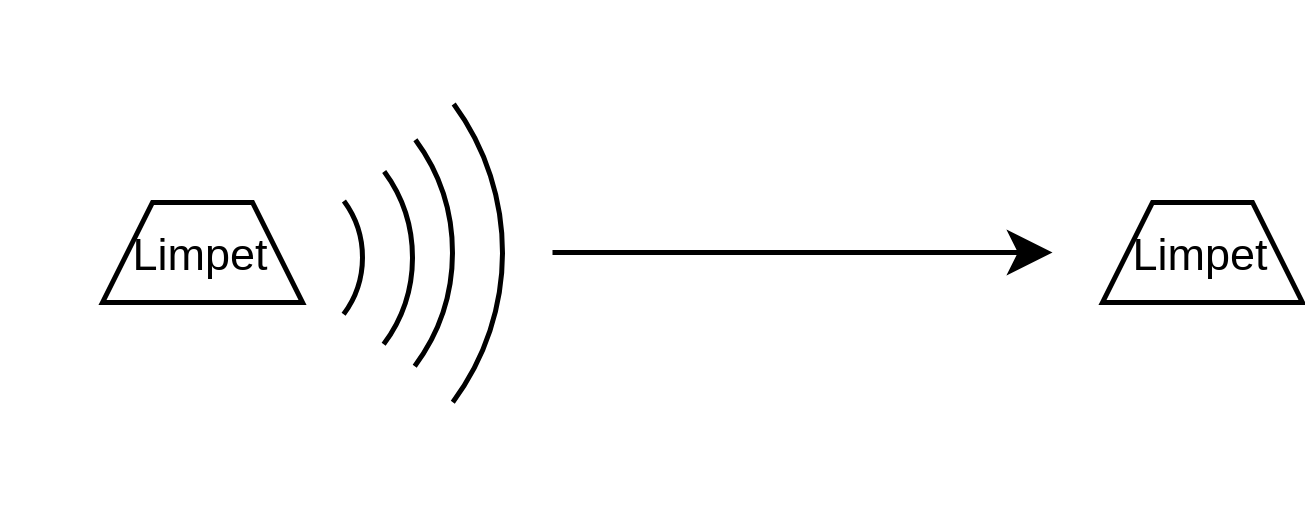
\includegraphics[width=0.71\textwidth]{images/limpetOneway}
	\caption{Limpet One-way Distance Measurement}
	\label{fig:limpetOneway}
\end{figure}

The one-way distance measurement relies on the RTC being accurate over long periods \cite{rtccomp}, from days to months, as a one meter difference in the distance measurement can be induced with a 3 millisecond difference between the RTC clocks. The RTC clock within the Nordic nRF52840 used in the limpets has a clock accuracy of $\pm$500ppm \cite{nrf52840}. The 500ppm results in a maximum shift in the RTC of ~$\pm$42 seconds in a day. 42 seconds equates to a measurement of distance incorrect by 13.9km, well beyond the acceptable error.\\

As can be seen the one-way distance measurement is not a suitable solution to the problem. The second approach that was designed was creating a virtual wall that bounces a sound between the limpets. This is achieved by when receiving a tone, a response is produced. The time between sending and receiving the time could then be used to calculate the distance without the need for reliable clocks over long periods. Figure \ref{fig:limpetTwoway} shows the process, step 1 send message, step 2 process message, step 3 send response.\\

\begin{figure}[H]
	\centering
	\noindent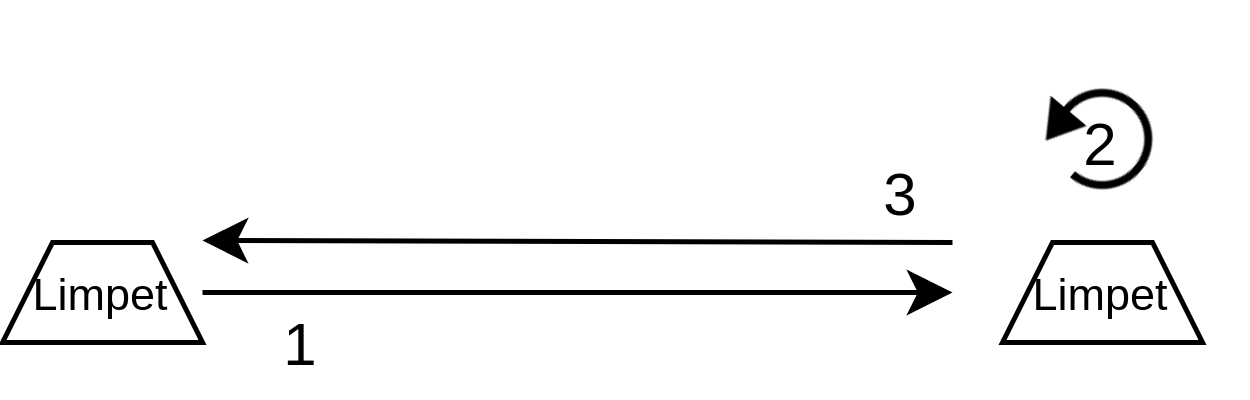
\includegraphics[width=0.71\textwidth]{images/limpetTwoway}
	\caption{Limpet Two-way Distance Measurement}
	\label{fig:limpetTwoway}
\end{figure}

The two-way distance measurement works if the processing for each limpet is know, this is possible to artificially increase processing to guarantee known periods. The known processing time can be subtracted from the time between sending and receiving. With the known two-way trip period the distance between the two limpets can be calculated. This provides a distance measurement between the two limpets to the limpet that started the measurement.\\

The two-way distance measurement can be improved upon by making it a 3-way measurement that provides a distance measurement for both limpets. Figure \ref{fig:limpetThreeway} shows the implementation of how the limpets would send messages.

\begin{figure}[H]
	\centering
	\noindent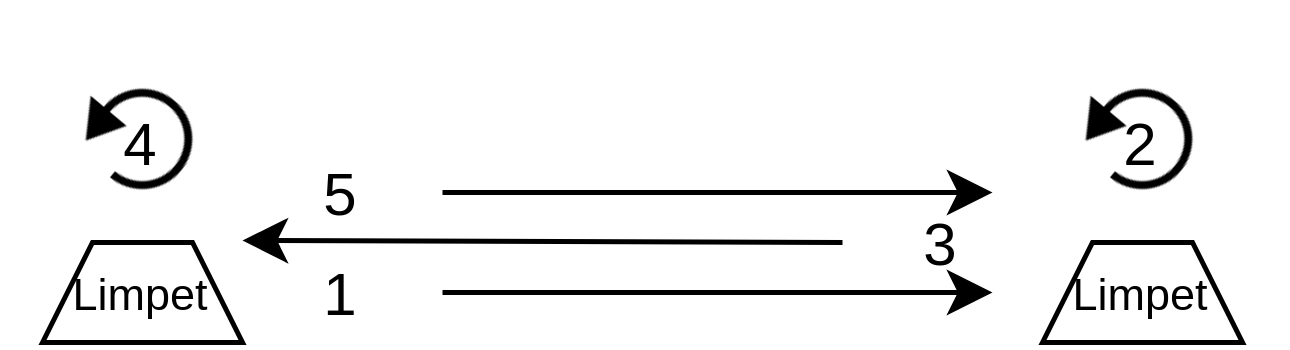
\includegraphics[width=0.71\textwidth]{images/limpetThreeway}
	\caption{Limpet Three-way Distance Measurement}
	\label{fig:limpetThreeway}
\end{figure}

\subsection{Multi-device Syncing}
A full network of Limpets could be in the the hundreds, as a consequence when a measurement is to be taken multiple Limpets could try to talk over each other. To remedy this an order of operations was constructed that decided on which Limpet was talking, and how the Limpet talked to others. This order is as follows:

\begin{itemize}
\item Initialise Decider
\item Identify Nearby
\item Distance Measurements
\item Information Distribution
\end{itemize}

A visual representation of the process can be seen in Figure \ref{fig:limpetHeirachy}.

\begin{figure}[H]
	\centering
	\noindent\includegraphics[width=0.71\textwidth]{images/limpetHeirachy}
	\caption{Limpet Multi-device Distance Measurement Process}
	\label{fig:limpetHeirachy}
\end{figure}

Figure \ref{fig:limpetHeirachy} Step 1 is the Initialising Decider operation. Initialising Decider is an operation that decides which Limpet should start making distance measurements. This could be decided based on the limpet with the lowest ID for example.\\

Step 2 is the Identify Nearby operation. Identify Nearby is an operation that identifies all nearby limpets that could possible hear it's distance measurement. This can be done through using the Limpets onboard Bluetooth capabilities or through the speaker and microphone.\\

Distance Measurements is an operation where the initial Limpet tells a device it is going to measure the distance between them. This is repeated until all Limpets that were identified have had the distances measured.\\

Information Distribution is an operation where all gathered distance measurements are provided to neighbouring Limpets as maximise the chance that distance measurements between Limpets are uploaded to a server. This operation also decides the next Limpet that will gather distance measurements, repeating the process.

\subsection{Mesh Generation}
\subsubsection{Background Research}
One of the final steps in the project is creating a 3-Dimensional mesh of all limpets in a network. Due to limitations of the measurements capable of being taken by the limpets, only the distance between limpets can be found and not orientation. This limitation meant that generating a 3D mesh of the limpet network wasn't a simple task.\\

Before doing research, the problems with only distance measurements and no direction were shown as to justify doing research. This was done by initially taking N points and seeing if arbitrary distances between all points can construct only one possible mesh with one know point.\\

Figure \ref{fig:3PMesh} shows the only possible combination for a 3 point mesh, with one originally known point. Figure \ref{fig:4PMesh} shows that there are at least two possible combinations, with one originally known point. As there is more than one possible combination for a four point mesh, research needs to be done into possible ways of generating a mesh of N points that is accurate to the real positions of the limpets relative to each other.\\

\begin{figure}[H]
	\centering
	\noindent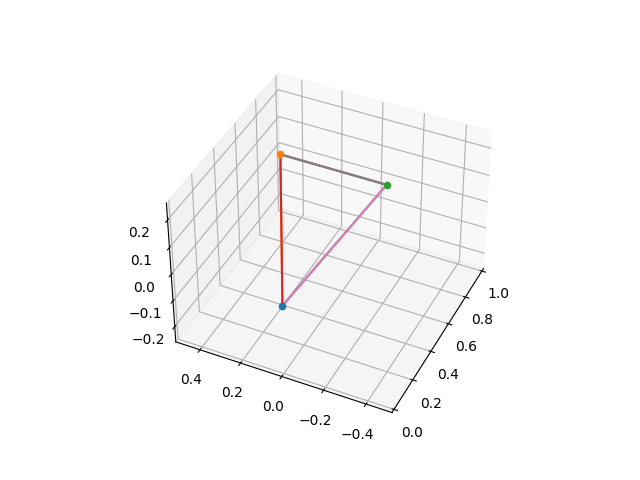
\includegraphics[width=0.49\textwidth]{images/3LimpetNet}
	\caption{Three Limpet Mesh Possible Configurations}
	\label{fig:3PMesh}
\end{figure}

\begin{figure}[H]
	\centering
	\noindent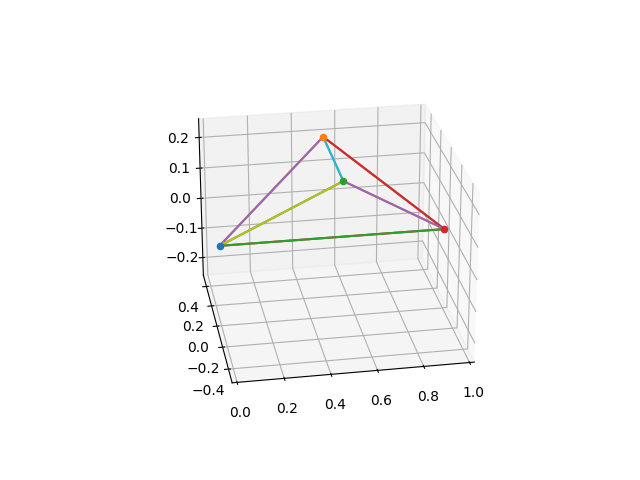
\includegraphics[width=0.49\textwidth]{images/4LimpetNet}
	\noindent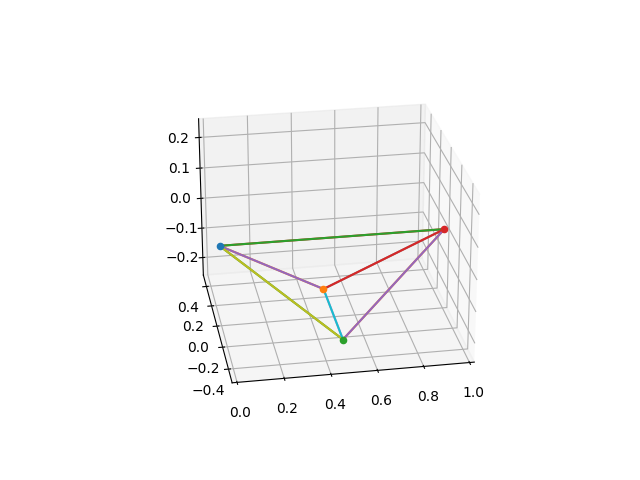
\includegraphics[width=0.49\textwidth]{images/4LimpetNetFlip}
	\caption{Four Limpet Mesh Possible Configurations}
	\label{fig:4PMesh}
\end{figure}

While researching, an existing system was discovered that found the location of an object based only on distance measurements between objects. The existing system was GPS Satellite Tracking. GPS uses four satellites which position are known relative to each other to find a fifth point with unknown location \cite{gps}. The same system which GPS uses with four known points to find the relative location of a unknown point can be implemented to generate a mesh.
\subsubsection{2D Mesh Generation}
To start, a 2D version of the full 3D mesh generation is useful to prove that the mesh generation would even be possible. Within a 2D system, to full define an unknown point's location, distance measurements are required from at least 3 known points. Figure \ref{fig:2d_mesh_ex} shows an example of a single step in 2D Mesh Generation with a 10\% distance measurement error. The left graph in Figure \ref{fig:2d_mesh_ex} shows the real locations for each of the points. Points 1,2, and 3 are known locations, and point 4 is the unknown location.

\begin{figure}[H]
	\centering
	\noindent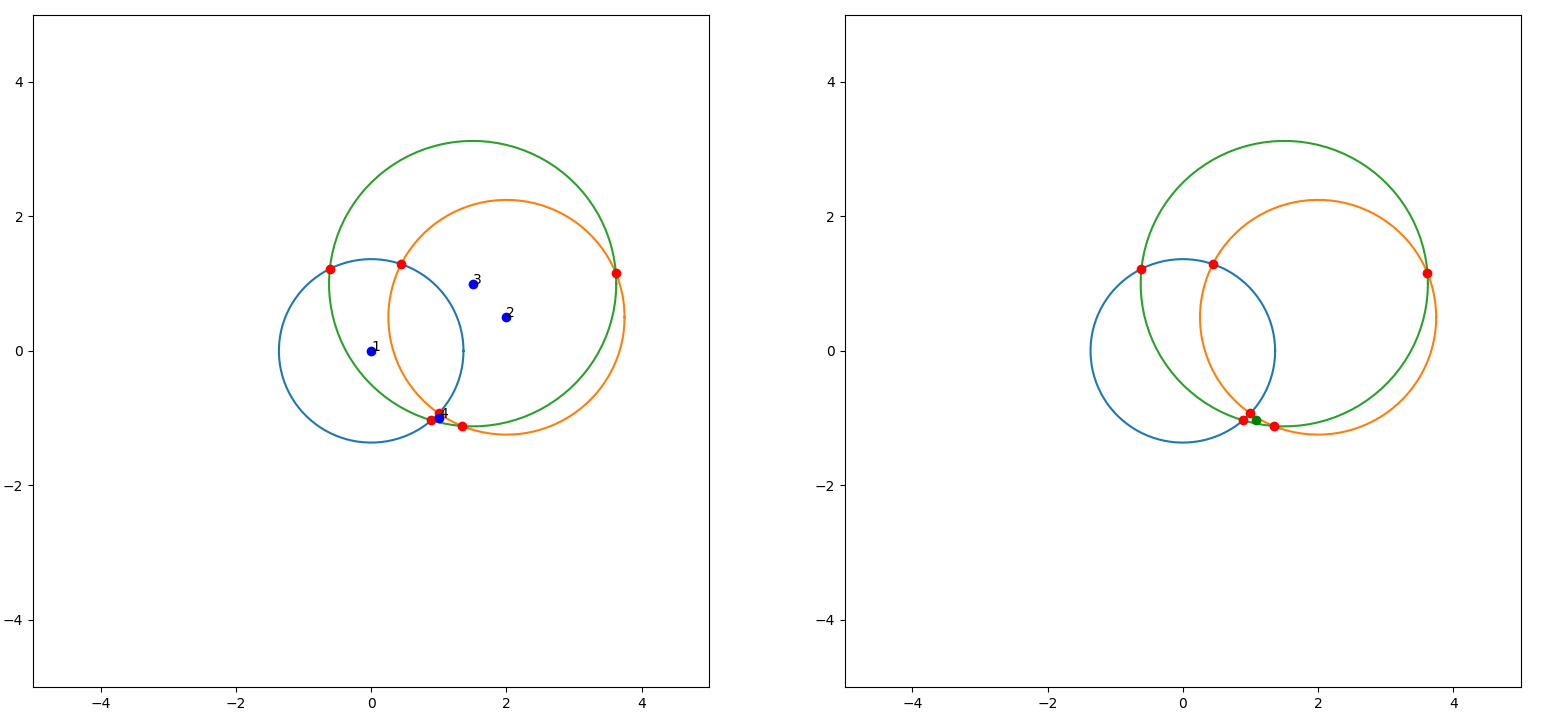
\includegraphics[width=0.8\textwidth]{images/2d_mesh_example.png}
	\caption{2D Mesh Generation Example}
	\label{fig:2d_mesh_ex}
\end{figure}

The circles in Figure \ref{fig:2d_mesh_ex} have a radius equal to the distance measurement between each known point and point 4. This means the circles show all possible locations that point 4 can be relative to the known points. To decrease the number of possible locations that point 4 could be in, the intersects of the circles are found. The intersects are shown by the red dots. The actual final location of where point 4 is can be found by looking at the largest cluster of intersects.\\

The predicted location of point 4 is shown in the right graph of Figure \ref{fig:2d_mesh_ex} as a green dot. As can be seen, the approximate location of point 4 can be found. Through testing, it can be noted that the closer two known points are, e.g. points 2 and 3, the greater error in predicted location of the unknown point. Overall, this simplistic implementation of 2D mesh generation suggests that 3D Mesh Generation is possible.

\subsubsection{3D Mesh Generation}
The approach to finding the location of an unknown point in the 3D mesh generation system is different from the 2D mesh generation method. Though the solution applied here can also be applied to the 2D mesh generation. A significant difference between the 2D mesh generation and 3D mesh generation is the quantity of points that need to be known to find an unknown point, this being 4 known points.\\

The approach is to use a root finding algorithm that finds the roots of a system of equations. Equation \ref{eg:gps_math} shows the system of equations that define the location of a location at $x, y, z$ based on the known points $x_n, y_n, z_n$ with distance measurements $d_n$. The reason to use a root finding algorithm is because the distance measurements will have an error, and root finding algorithms can handle a degree of error.\\

\begin{equation} \label{eg:gps_math}
	\begin{matrix}
		\sqrt{(x-x_1)^2+(y-y_1)^2+(z-z_1)^2} = d_1\\
		\sqrt{(x-x_2)^2+(y-y_2)^2+(z-z_2)^2} = d_2\\
		\sqrt{(x-x_3)^2+(y-y_3)^2+(z-z_3)^2} = d_3\\
		\sqrt{(x-x_4)^2+(y-y_4)^2+(z-z_4)^2} = d_4
	\end{matrix}
\end{equation}\\

Figure \ref{fig:3d_mesh_ex} shows an example of the implemented system, using 4 known points to find a 5\textsuperscript{th} unknown point. The spheres are used to indicate the possible locations of the unknown point relative to each individual known point. The code used to achieve these examples is shown in Appendix \ref{sec:tob_code_append}.

\begin{figure}[H]
	\centering
	\noindent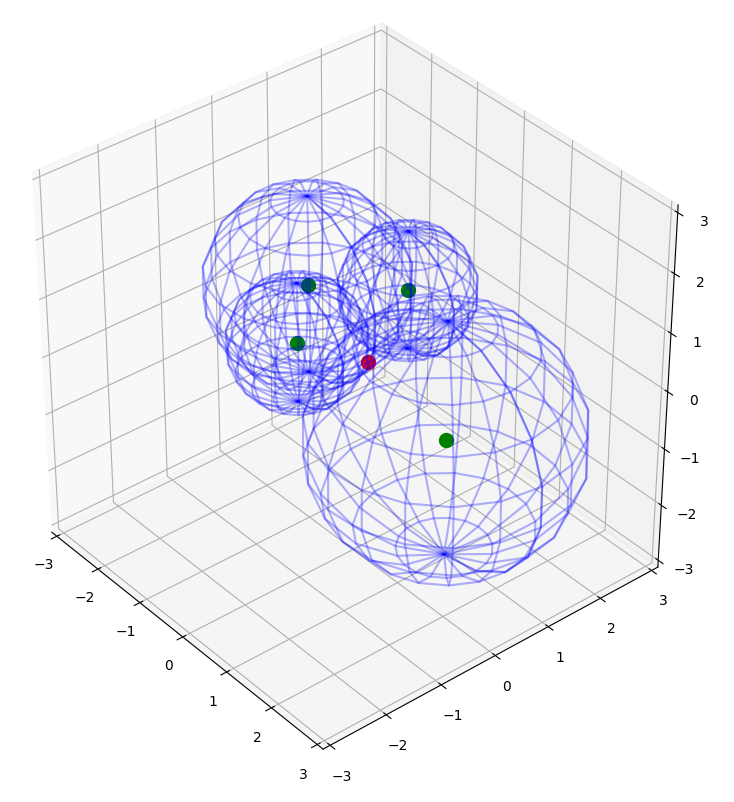
\includegraphics[width=0.4\textwidth]{images/3d_mesh_sph.png}
	\caption{3D Mesh Generation Example}
	\label{fig:3d_mesh_ex}
\end{figure}


